\chapter{Claude Shannon et la compression des données}
\label{chap-shannon}
\chapteroverview{Combien de bits faut-il pour conserver un message sans perdre d'information ? La théorie de Shannon relie cette question aux probabilités des symboles qui composent le message. À partir d'une petite image en niveaux de gris, nous introduisons les codes binaires, expliquons le décodage sans ambiguïté et précisons le rôle de l'entropie dans la compression.}

\section{Données numériques et codage}
Textes, sons, images et vidéos sont stockés et transmis sous forme de suites de bits : des chiffres binaires $\RE{0}$ et $\RE{1}$. Avant de choisir cette représentation, on décrit les données par des \emph{symboles}, par exemple les lettres d'un texte ou les valeurs des pixels d'une image. Une méthode de compression sans perte remplace une suite de symboles par une représentation binaire plus courte dont on peut retrouver exactement la suite initiale.

Les travaux de Shannon~\cite{Shannon1948,shannon1949} ont établi des limites fondamentales pour la représentation et la transmission de l'information. Il convient de distinguer plusieurs opérations :
\begin{itemize}
\item L'\emph{échantillonnage} relève les valeurs d'un signal continu en certains points ou instants. La \emph{quantification} remplace ensuite ces valeurs par des éléments d'un ensemble fini.
\item Le \emph{codage de source}, étudié dans ce chapitre, recherche une représentation compacte des symboles obtenus.
\item Le \emph{codage de canal} ajoute de la redondance pour détecter ou corriger des erreurs de transmission. La protection contre des modifications malveillantes relève d'un problème de sécurité distinct.
\end{itemize}
L'échantillonnage et la quantification peuvent supprimer de l'information. Le codage étudié ici est sans perte par rapport aux symboles déjà acquis. Cette distinction est essentielle lorsque l'on parle de compresser une photographie ou un enregistrement sonore.

\section{Codage et décodage}
\subsection{Une petite image en niveaux de gris}
Une image en niveaux de gris est un tableau de pixels. Pour simplifier, considérons quatre valeurs possibles : $\BL{0}$ pour le noir, $\BL{1}$ pour le gris foncé, $\BL{2}$ pour le gris clair et $\BL{3}$ pour le blanc. Les mêmes idées s'appliquent à un alphabet plus grand, comme les 256 valeurs d'une image en niveaux de gris sur huit bits, ainsi qu'aux composantes d'une image en couleur.

La figure~\ref{fig-image-zoom} représente une fleur et l'agrandissement d'un carré de $5\times5$ pixels. En lisant ses 25 valeurs dans l'ordre indiqué, on obtient
\begin{equation}\label{eq-pixel-message}
 (\BL{0,1,3,2,0,3,2,2,1,2,2,1,1,2,2,2,1,1,2,2,2,1,1,2,1}).
\end{equation}
\myfig{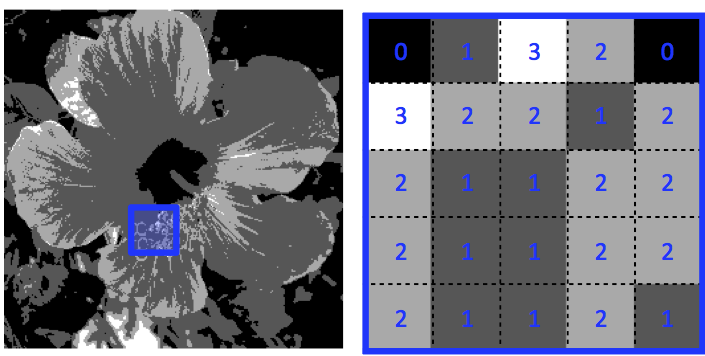
\includegraphics[width=.60\linewidth]{codage/codage-pxl}}
{fig-image-zoom}{Une image à quatre niveaux de gris et l'agrandissement d'un carré de $5\times5$ pixels.}

\subsection{Codage à longueur fixe}
Sauf si la longueur du message est connue à l'avance, on impose des mots de code non vides.
Un \emph{mot de code} est la suite de bits associée à un symbole. On peut choisir
\[
 \BL{0}\mapsto\RE{00},\qquad \BL{1}\mapsto\RE{01},\qquad
 \BL{2}\mapsto\RE{10},\qquad \BL{3}\mapsto\RE{11}.
\]
Les quatre mots ont une longueur égale à deux : il s'agit d'un code \emph{à longueur fixe}, également appelé code uniforme. Coder un message consiste à concaténer les mots de code de ses symboles. Par exemple,
\[
 (\BL{0,1,3})\longmapsto(\RE{00},\RE{01},\RE{11})\longmapsto\RE{000111}.
\]
Le message complet~\eqref{eq-pixel-message} devient
\[
 \RE{\mathtt{00011110001110100110100101101010010110101001011001}}.
\]
Sa longueur totale vaut $\overline{L}=25\times2=50$ bits. Ce calcul porte sur les valeurs des pixels codées ; un fichier peut aussi contenir les dimensions de l'image, une table de codage et d'autres métadonnées.

Pour un alphabet de $N\ge2$ symboles, un code binaire à longueur fixe $\ell$ existe exactement lorsque $2^\ell\geq N$ : il faut disposer d'au moins autant de mots binaires distincts que de symboles. La plus petite longueur possible est donc
\[
 \ell=\lceil\log_2 N\rceil.
\]
Lorsque $N=2^\ell$, tous les mots binaires sont utilisés. Pour $N=8$, par exemple, ce sont $000$, $001$, $010$, $011$, $100$, $101$, $110$, $111$, de longueur $\ell=3$.

Le logarithme en base deux est défini pour $x>0$ par $\log_2x=\ln x/\ln2$. Il vérifie $\log_2(1/x)=-\log_2x$ ; en particulier,
\[
 \log_2(1/4)=-\log_2 4=-2.
\]
L'arrondi à l'entier supérieur dans la formule de $\ell$ est indispensable lorsque $N$ n'est pas une puissance de deux.

\subsection{Codage à longueur variable}
On peut réduire le nombre moyen de bits en attribuant des mots plus courts aux symboles fréquents. Considérons le code
\begin{equation}\label{eq-prefix-example}
 \BL{0}\mapsto\RE{001},\qquad \BL{1}\mapsto\RE{01},\qquad
 \BL{2}\mapsto\RE{1},\qquad \BL{3}\mapsto\RE{000}.
\end{equation}
La suite $(\BL{0,1,3})$ devient $\RE{00101000}$ et le message complet s'écrit
\[
 \RE{\mathtt{001010001001000110111010111101011110101101}}.
\]
Cette suite comporte 42 bits. Sa \emph{longueur moyenne par symbole} vaut
\[
 L=\frac{\overline{L}}{25}=\frac{42}{25}=1{,}68\ \text{bits}.
\]
Pour ce message, le code est plus économique que le code à longueur fixe. Il ne l'est pas nécessairement pour tout message : une suite composée surtout des symboles $\BL{0}$ et $\BL{3}$ demanderait près de trois bits par symbole.

\subsection{Codes préfixes et décodage sans ambiguïté}
Un code est \emph{uniquement décodable} si deux suites finies de symboles différentes ne produisent jamais la même suite de bits. Un code à longueur fixe dont les mots sont distincts possède cette propriété : il suffit de découper le message en blocs de $\ell$ bits, puis de lire la table de codage en sens inverse.

Pour un code à longueur variable, il ne suffit pas que les mots soient distincts. Ainsi, le code
\[
 \BL{0}\mapsto\RE{0},\quad \BL{1}\mapsto\RE{10},\quad
 \BL{2}\mapsto\RE{110},\quad \BL{3}\mapsto\RE{101}
\]
est ambigu : $\RE{1010}=\RE{10}\,\RE{10}=\RE{101}\,\RE{0}$ représente aussi bien $(\BL{1,1})$ que $(\BL{3,0})$.

Une condition suffisante pour assurer l'unicité du décodage est qu'aucun mot ne soit un préfixe propre d'un autre. On parle alors de \emph{code préfixe}. Le code~\eqref{eq-prefix-example} vérifie cette condition. Chaque mot est reconnu dès que son dernier bit est lu :
\[
 \underbrace{\RE{001}}_{\BL{0}}\;
 \underbrace{\RE{01}}_{\BL{1}}\;
 \underbrace{\RE{000}}_{\BL{3}}\;
 \underbrace{\RE{1}}_{\BL{2}}\;\cdots.
\]
Les espaces servent ici à expliquer le décodage ; ils ne sont pas transmis.

La condition de préfixe est suffisante, mais pas nécessaire. Le code $A\mapsto0$, $B\mapsto01$ est uniquement décodable, bien que $0$ soit un préfixe de $01$. Chaque $1$ doit être associé au $0$ qui le précède : le message complet ne possède donc qu'un seul découpage. Après avoir lu un $0$, le décodeur doit néanmoins regarder la suite pour décider s'il représente $A$ ou commence $B$. D'autres codes non préfixes peuvent imposer des décisions différées ou des retours en arrière ; les codes préfixes évitent cette difficulté.

\subsection{Codes et arbres binaires}\label{sec-arbres}
Le mot vide est la racine d'un arbre binaire. Ajouter un $0$ ou un $1$ revient à choisir son fils gauche ou son fils droit. Un mot de longueur $\ell$ se trouve à la profondeur $\ell$ ; l'arbre complet de profondeur $\ell$ possède donc $2^\ell$ feuilles et $\ell+1$ niveaux, racine comprise.

\myfig{\tabDeux{
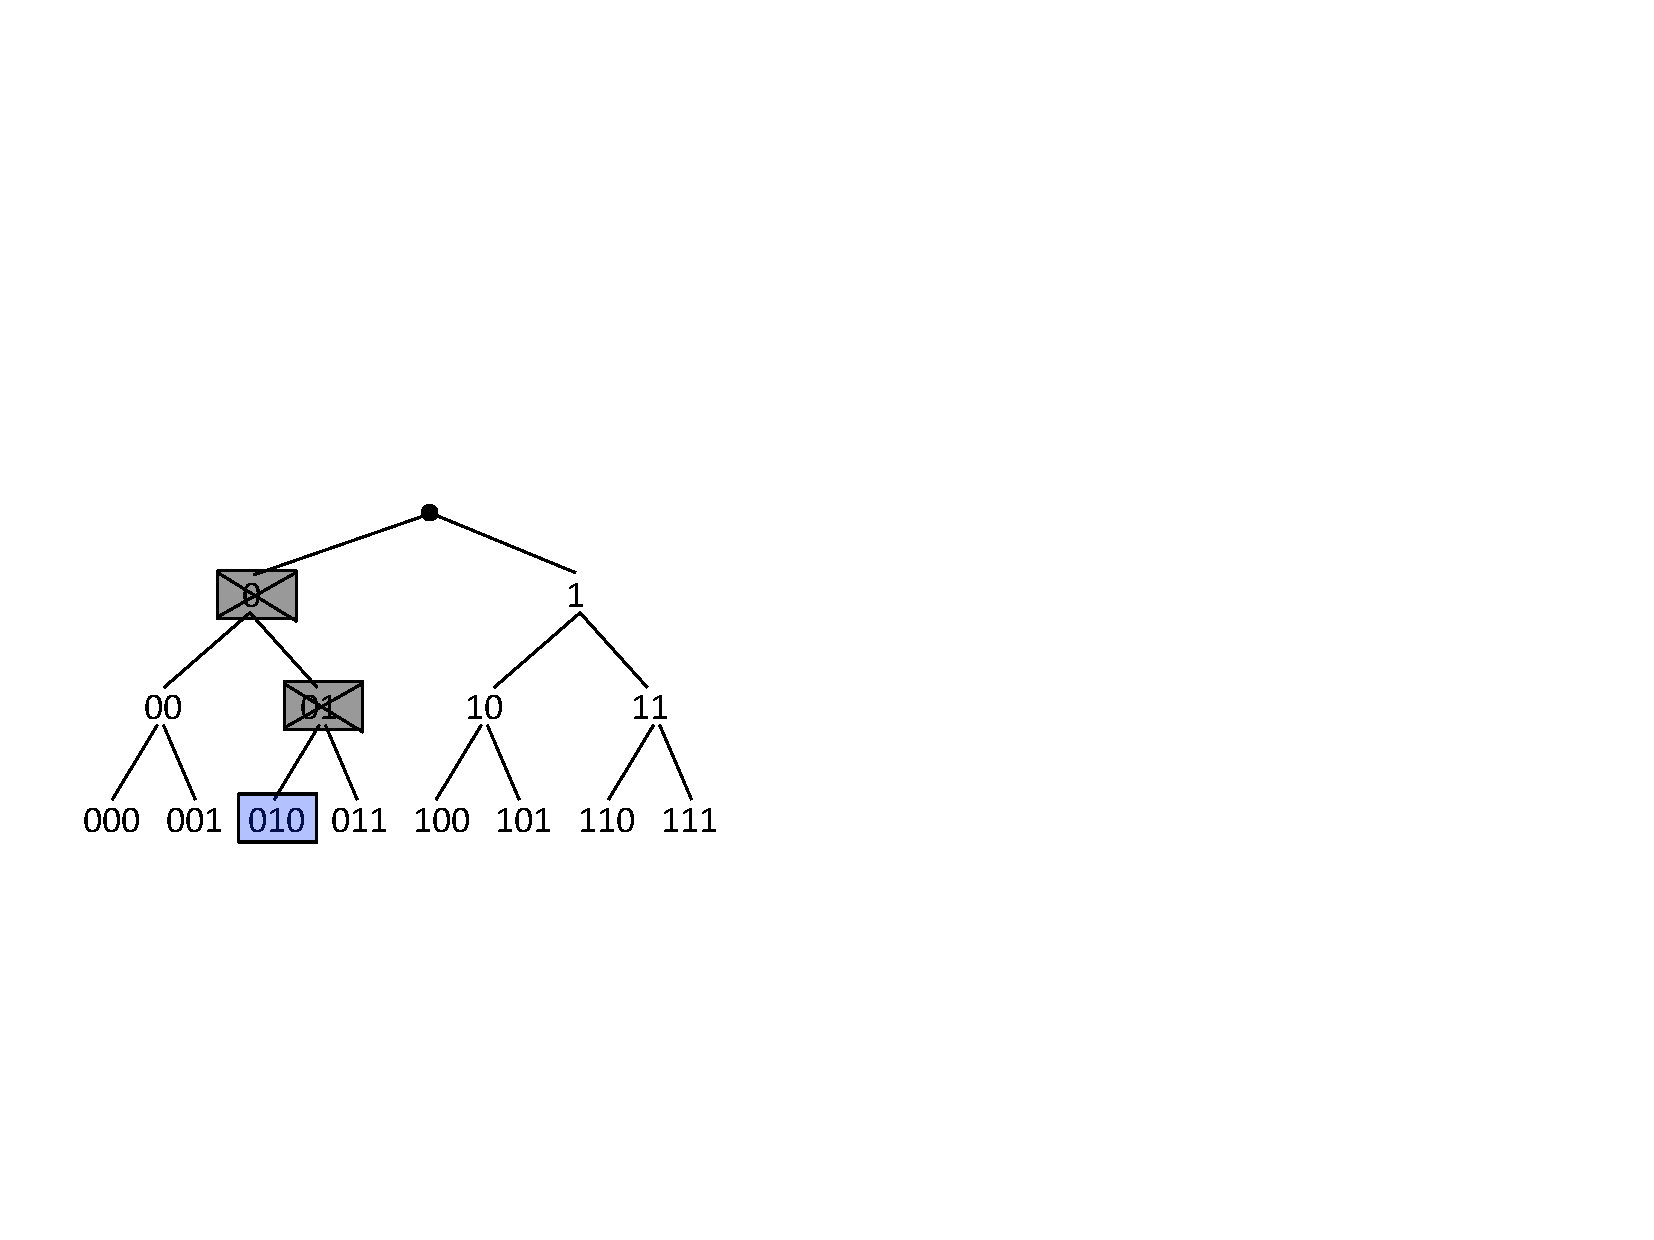
\includegraphics[width=.42\linewidth]{arbres/codage-prefixe}&
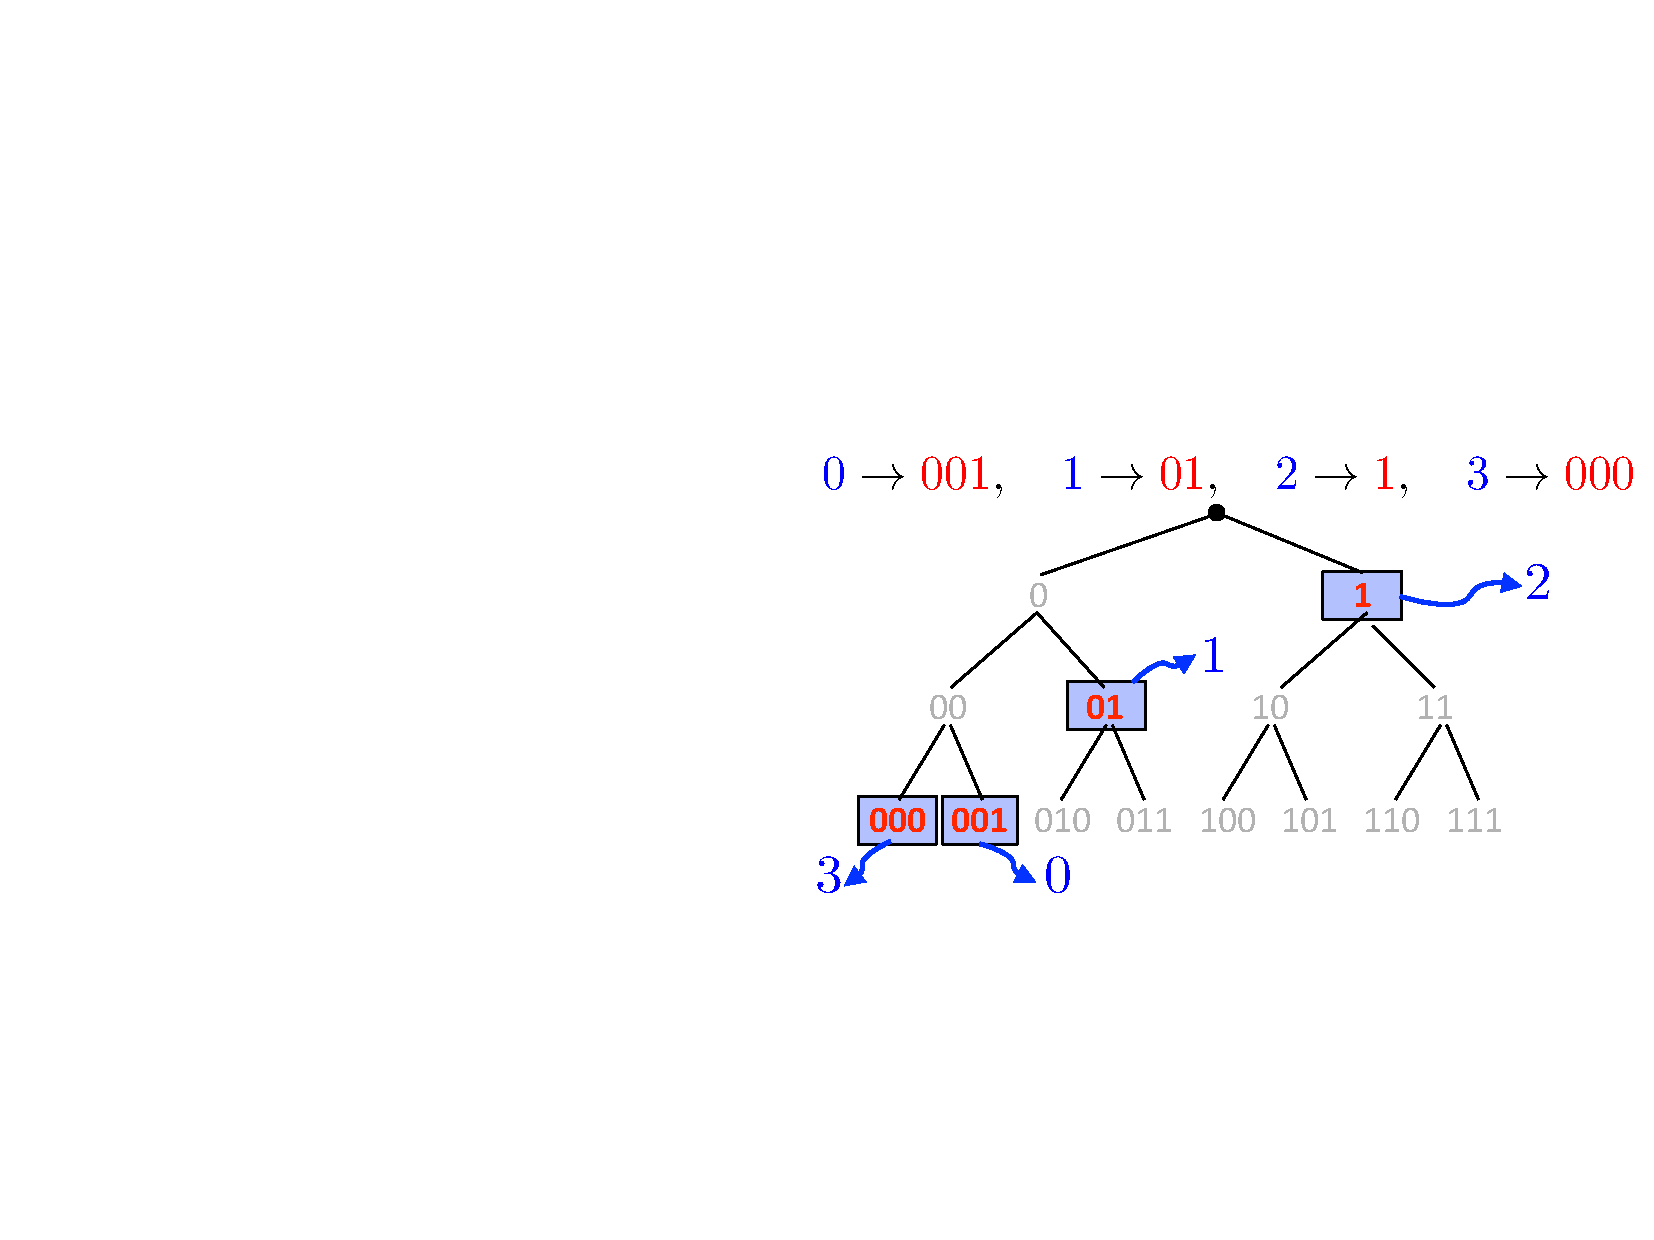
\includegraphics[width=.42\linewidth]{arbres/arbre-exemple}}}
{fig-trees}{L'arbre binaire complet de profondeur trois (à gauche) et le sous-arbre d'un code préfixe (à droite).}

Dans un code préfixe, aucun nœud choisi comme mot de code n'est l'ancêtre d'un autre. Les nœuds choisis sont donc les feuilles de l'arbre formé par leurs chemins depuis la racine. Pour décoder, on part de la racine et l'on suit une arête par bit lu. Quand on atteint une feuille portant un mot de code, on émet le \emph{symbole} correspondant, puis on revient à la racine. Cette procédure rend le décodage immédiat et sans ambiguïté.

\section{Entropie et borne de Shannon}
\subsection{Un modèle probabiliste}
La qualité d'un code dépend des messages auxquels on l'applique. Un modèle probabiliste permet d'expliciter cette dépendance. Soit $V$ un symbole aléatoire à valeurs dans $\{0,\ldots,N-1\}$, de probabilités
\[
 p_v=\mathbb{P}(V=v),\qquad p_v\geq0,\qquad \sum_{v=0}^{N-1}p_v=1.
\]
Le modèle le plus simple produit une suite de symboles indépendants ayant tous cette distribution. L'indépendance est une hypothèse sur la source, et non une propriété assurée par l'algorithme de codage.

Pour un message observé, on peut estimer les probabilités par les \emph{fréquences empiriques}. Le message~\eqref{eq-pixel-message} contient 2 zéros, 9 uns, 12 deux et 2 trois. Sa distribution empirique est
\[
 p=(2/25,\;9/25,\;12/25,\;2/25).
\]
Utiliser ces fréquences comme probabilités constitue un choix de modélisation. Si le décodeur ne connaît pas déjà le modèle ou la table de codage retenus, il faut également transmettre les informations qui les décrivent.

\subsection{Entropie}
L'\emph{entropie} de $V$, mesurée en bits, est
\begin{equation}\label{eq-entropy}
 H(V)=-\sum_{v=0}^{N-1}p_v\log_2p_v.
\end{equation}
Un symbole de probabilité $p_v>0$ apporte une information égale à $-\log_2p_v$. L'entropie est la moyenne de cette quantité. La convention $0\log_2 0=0$ signifie que les symboles impossibles ne contribuent pas à la somme ; elle est cohérente avec $\lim_{x\downarrow0}x\log_2x=0$.

Comme $-\log_2p_v\geq0$, l'entropie est positive ou nulle. Plus précisément,
\[
 0\leq H(V)\leq\log_2N.
\]
Les valeurs extrêmes décrivent deux modèles utiles :
\begin{itemize}
\item \textbf{Aucune incertitude.} Si $p_1=1$, tous les symboles valent $1$ et $H(V)=0$. Le message est donc une suite de uns.
\item \textbf{Incertitude maximale.} Si $p_v=1/N$ pour tout $v$, alors $H(V)=\log_2N$. Avec quatre symboles équiprobables, cette valeur est de deux bits. Un message aléatoire produit par ce modèle ne contient pas nécessairement autant d'occurrences de chaque symbole.
\item \textbf{Une situation intermédiaire.} Pour la distribution empirique précédente,
\[
 H(V)=-2\frac{2}{25}\log_2\frac{2}{25}
       -\frac{9}{25}\log_2\frac{9}{25}
       -\frac{12}{25}\log_2\frac{12}{25}
       \simeq1{,}6219\ \text{bits}.
\]
\end{itemize}
\myfig{\tabTrois{
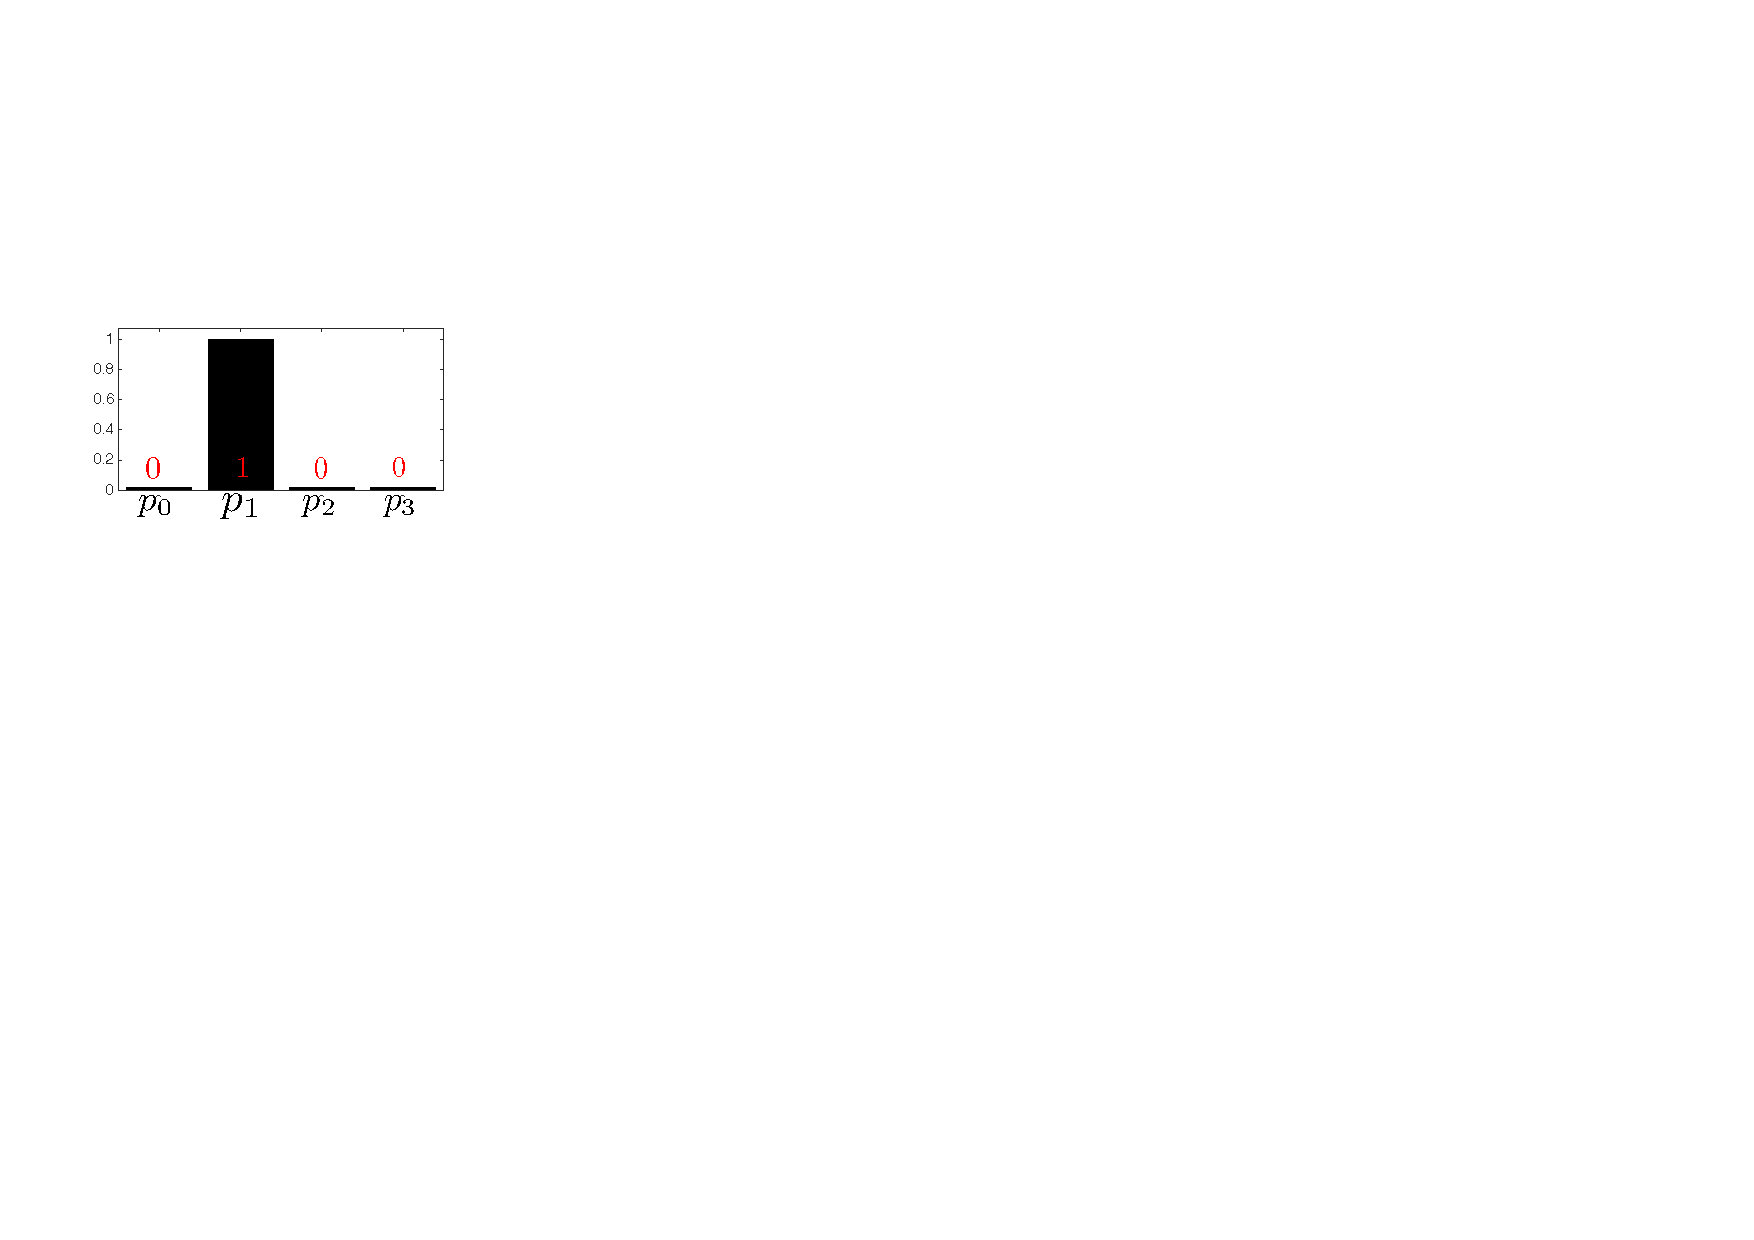
\includegraphics[width=.30\linewidth]{entropie/histo-1}&
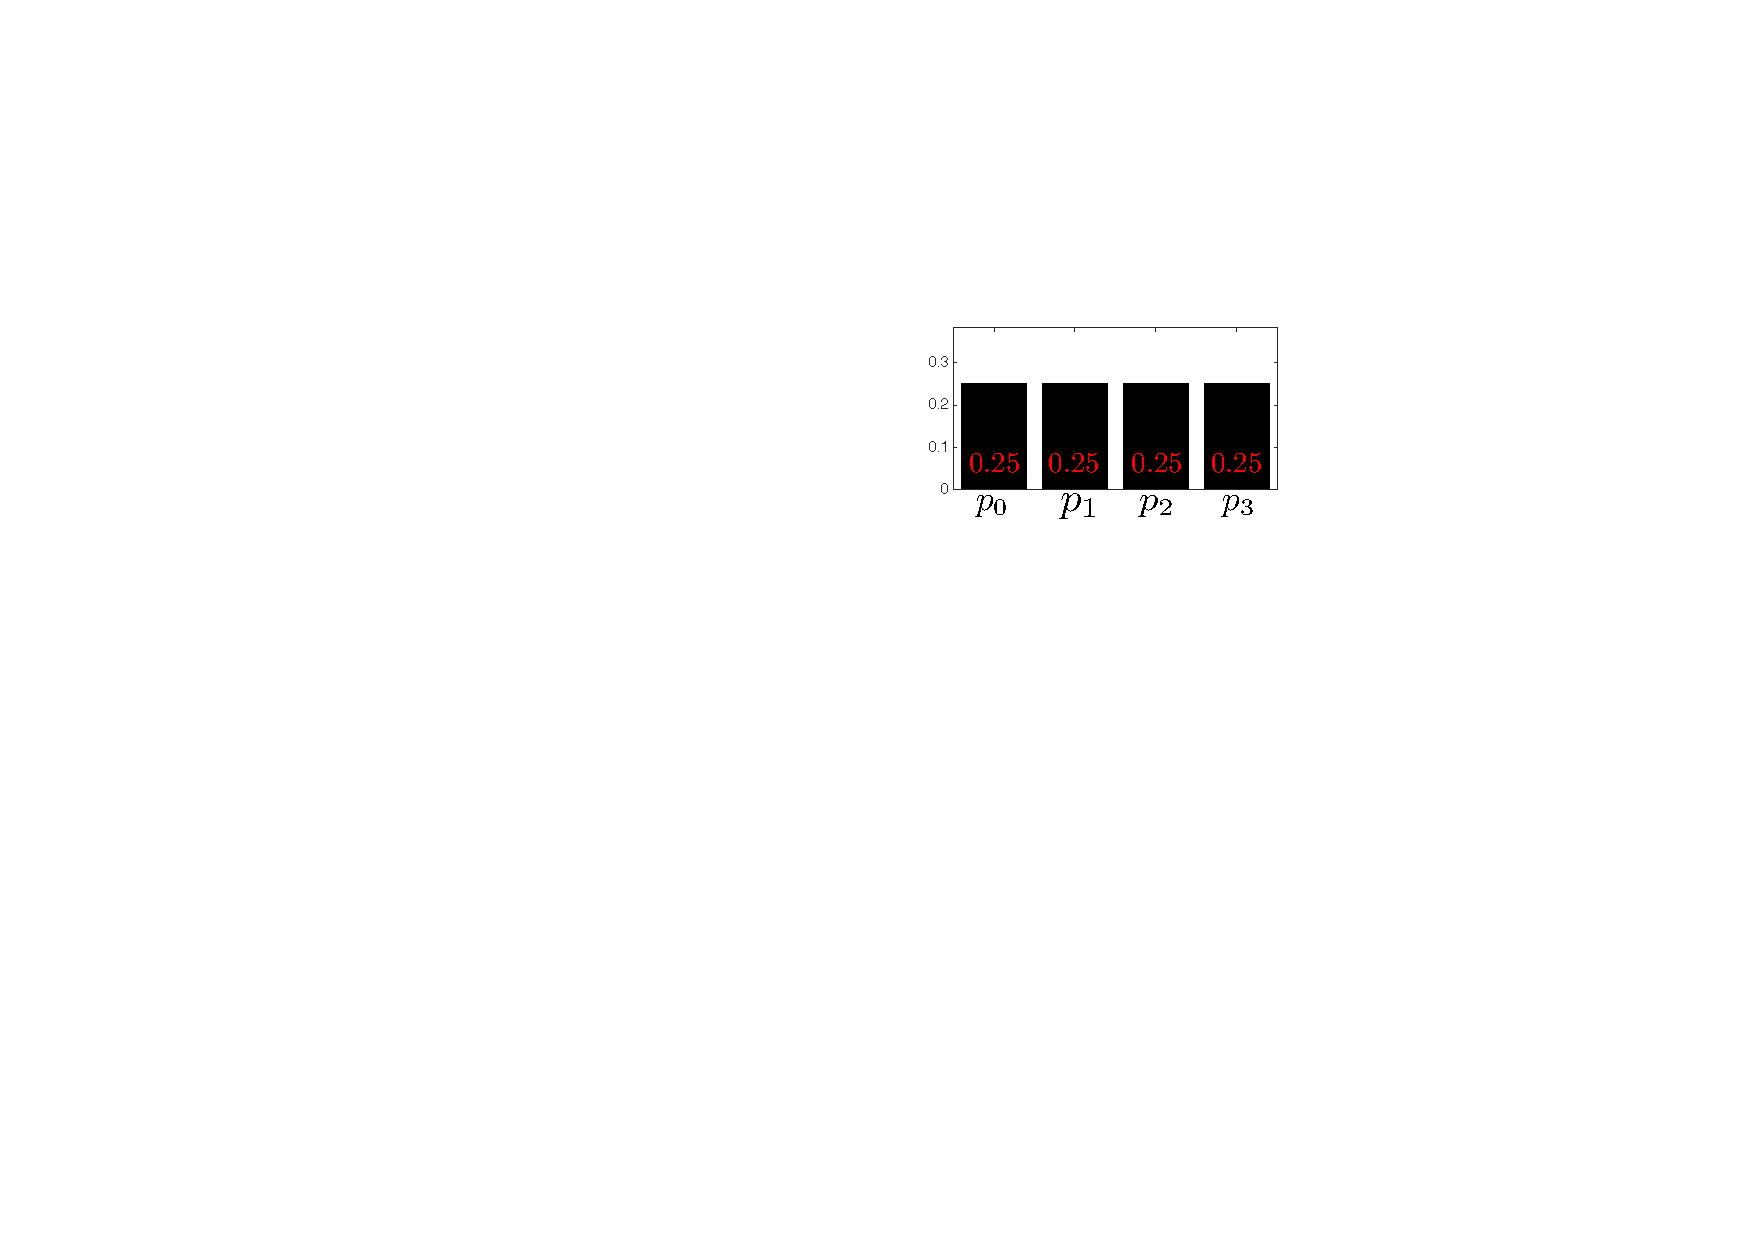
\includegraphics[width=.30\linewidth]{entropie/histo-3}&
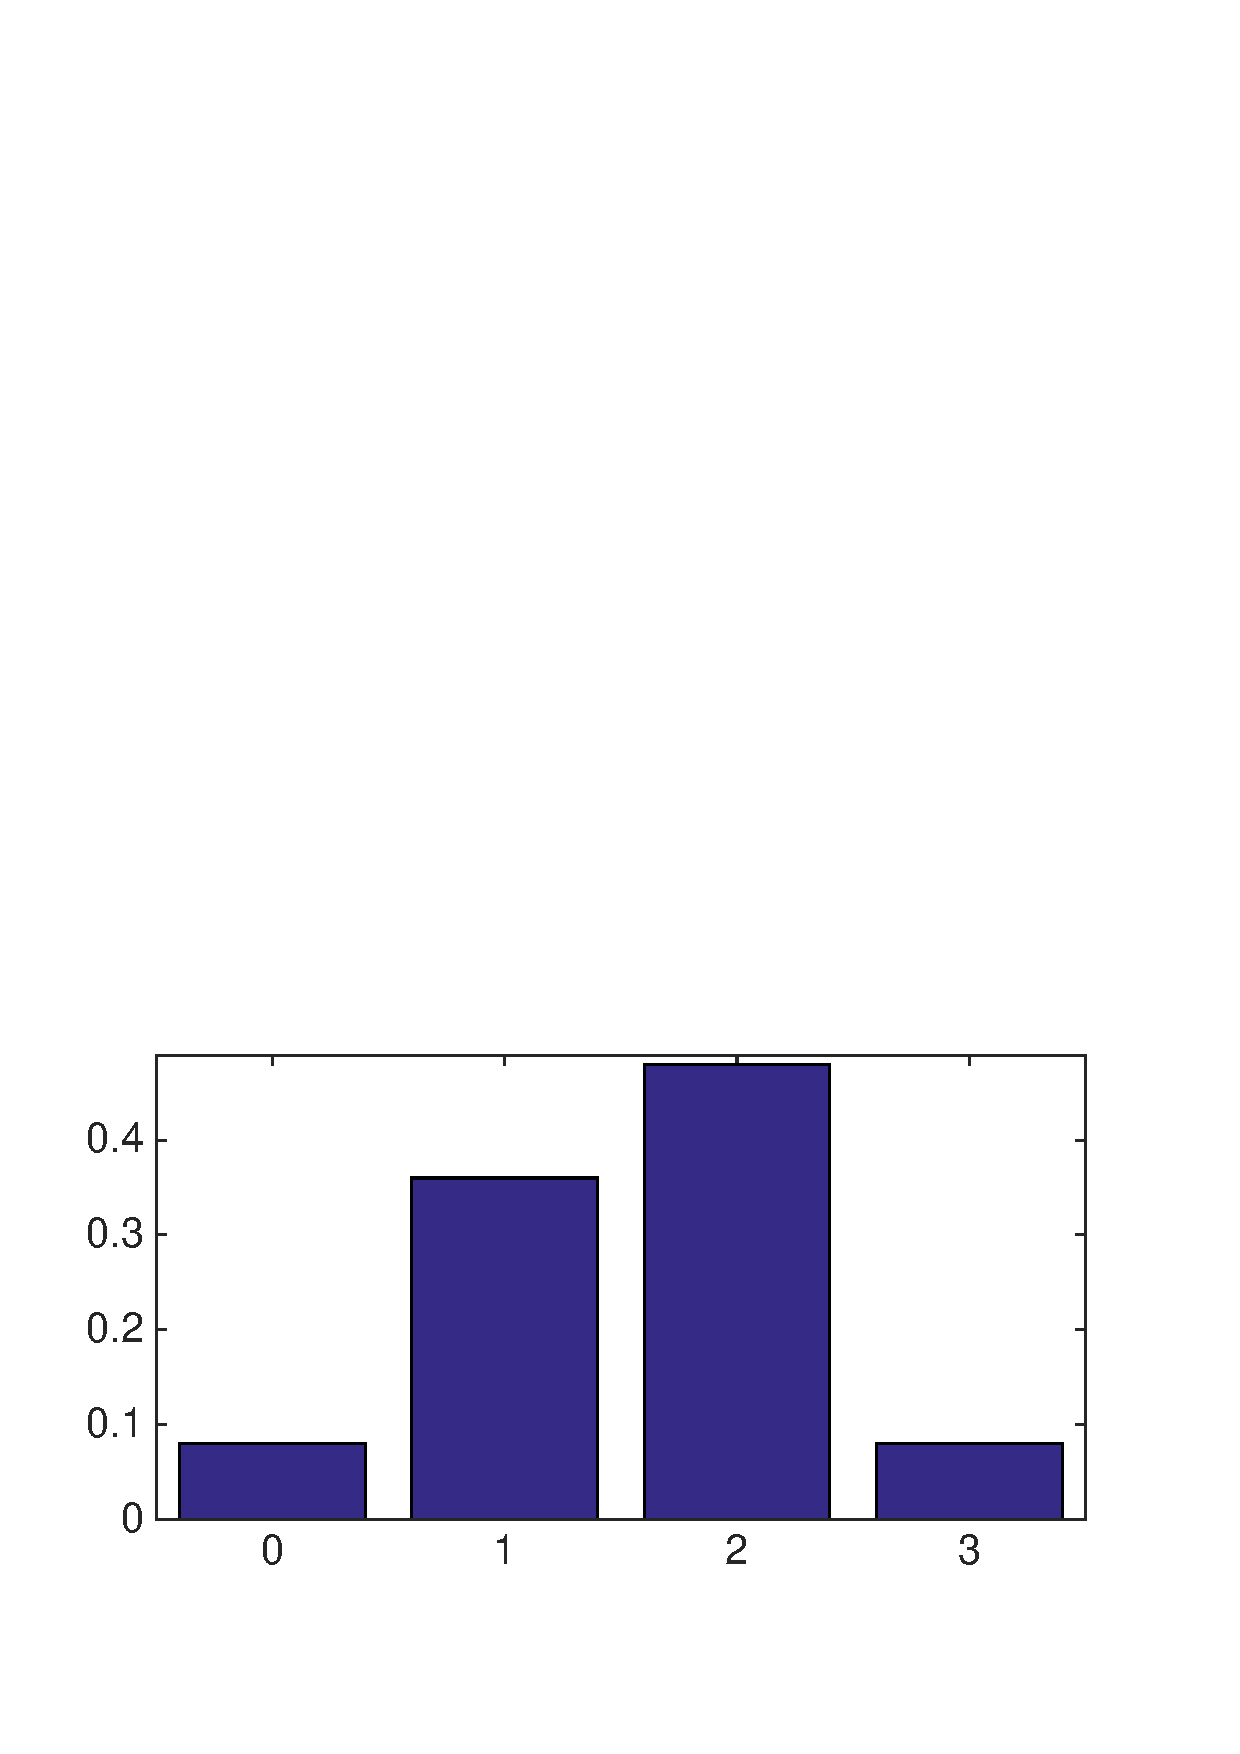
\includegraphics[width=.30\linewidth]{entropie/histo-sub}\\
$H(V)=0$&$H(V)=2$&$H(V)\simeq1{,}62$}}
{fig-histo-entropy}{Une distribution déterministe, la distribution uniforme sur quatre symboles et la distribution empirique du message de 25 pixels.}

\subsection{Longueur moyenne d'un code}
Notons $c_v$ le mot de code du symbole $v$ et $\ell_v$ sa longueur. Le nombre moyen de bits par symbole est
\[
 L(c)=\mathbb{E}[\ell_V]=\sum_v p_v\ell_v.
\]
Pour le code~\eqref{eq-prefix-example}, les longueurs sont $(3,2,1,3)$, d'où
\[
 L(c)=\frac{2\times3+9\times2+12\times1+2\times3}{25}
     =\frac{42}{25}=1{,}68.
\]
Si $p$ est la distribution empirique d'un message fini, cette formule donne aussi sa longueur moyenne exacte. Si $p$ décrit un modèle de source, il s'agit d'une espérance.

\subsection{La borne inférieure de l'entropie}
Tout code binaire préfixe vérifie la borne de Shannon~\cite{Shannon1948}
\begin{equation}\label{eq-shannon-bound}
 H(V)\leq L(c).
\end{equation}
En voici une courte preuve. Soit $m$ la plus grande longueur d'un mot de code. Un mot de longueur $\ell_v$ possède $2^{m-\ell_v}$ descendants à la profondeur $m$. Pour les mots d'un code préfixe, ces ensembles de descendants sont disjoints, donc
\[
 \sum_v2^{m-\ell_v}\leq2^m,
 \qquad Z\eqdef\sum_v2^{-\ell_v}\leq1.
\]
C'est l'inégalité de Kraft. Posons $q_v=2^{-\ell_v}/Z$. Alors $\sum_vq_v=1$ et $\ell_v=-\log_2q_v-\log_2Z$, ce qui donne
\[
 \begin{aligned}
 L(c)-H(V)
 &=\sum_{v:p_v>0}p_v\log_2\frac{p_v}{q_v}-\log_2Z\\
 &\geq\sum_{v:p_v>0}p_v\log_2\frac{p_v}{q_v}\geq0.
 \end{aligned}
\]
La dernière somme est la divergence de Kullback--Leibler. Sa positivité découle de $\ln t\leq t-1$ : en appliquant cette inégalité à $t=q_v/p_v$ puis en sommant, on obtient $\sum p_v\ln(q_v/p_v)\leq\sum_{p_v>0}q_v-1\leq0$.

La borne porte sur une \emph{moyenne} ; elle n'impose pas séparément $\ell_v\geq-\log_2p_v$ pour chaque symbole. Les nombres réels $-\log_2p_v$ fournissent néanmoins des longueurs cibles utiles : une probabilité \emph{plus grande} donne une longueur cible plus petite. Pour une distribution uniforme sur $2^\ell$ symboles, le code à longueur fixe atteint exactement la borne. Pour d'autres tailles d'alphabet, l'intégralité des longueurs peut empêcher l'égalité.

\subsection{Codage de Huffman et codage par blocs}
L'algorithme de Huffman~\cite{Huffman52} construit un code préfixe de longueur moyenne minimale pour une distribution finie donnée. Les symboles de probabilité nulle sont omis de l’alphabet effectif. Pour une source ayant au moins deux symboles de probabilité strictement positive, cette longueur vérifie
\[
 H(V)\leq L(c)<H(V)+1.
\]
On peut comprendre la borne supérieure en arrondissant chaque longueur cible à l'entier supérieur : $\ell_v=\lceil-\log_2p_v\rceil$. Ces longueurs vérifient l'inégalité de Kraft et peuvent être réalisées par un code préfixe. Leur moyenne est strictement inférieure à $H(V)+1$, et le code de Huffman fait au moins aussi bien.

Pour réduire le surcoût par symbole, on peut coder des blocs de $n$ symboles indépendants. Leur entropie vaut $H(V_1,\ldots,V_n)=nH(V)$. Un code par blocs approprié a donc une longueur moyenne $L_n$ telle que
\[
 H(V)\leq\frac{L_n}{n}<H(V)+\frac1n.
\]
Le débit tend ainsi vers l'entropie lorsque la taille des blocs augmente. Le codage arithmétique~\cite{RissanenLangdon79} met en œuvre des idées voisines sans mémoriser une table de mots de code de taille exponentielle. Pour les messages finis, il subsiste des surcoûts liés au modèle, à la terminaison et à la précision numérique.

Si une source n'admet qu'un seul symbole, son entropie est nulle. Lorsque ce symbole et la longueur du message sont connus, aucun bit de contenu n'est nécessaire. Imposer un mot de code non vide coûterait au contraire au moins un bit par symbole. Il faut donc préciser les conventions de délimitation du message et l'alphabet effectivement utilisé.

\subsection{Exploiter la dépendance entre pixels}\label{sec-information-transform}
Les pixels voisins d'une image sont généralement dépendants. Un modèle qui traite les symboles séparément ignore cette structure. Une transformation des données avant le codage permet souvent de mieux l'exploiter.

Indexons les $P$ pixels par $v_0,\ldots,v_{P-1}$ et définissons
\[
 d_i=v_i-v_{i-1},\qquad 1\leq i\leq P-1.
\]
Conservons $v_0$ ainsi que les différences. La transformation
\[
 (v_0,\ldots,v_{P-1})\longmapsto(v_0,d_1,\ldots,d_{P-1})
\]
est bijective, car $v_i=v_0+\sum_{j=1}^i d_j$. Dans une région presque constante, la plupart des différences sont nulles ou petites. Pour des pixels à quatre niveaux, elles appartiennent à $\{-3,-2,-1,0,1,2,3\}$.
\myfig{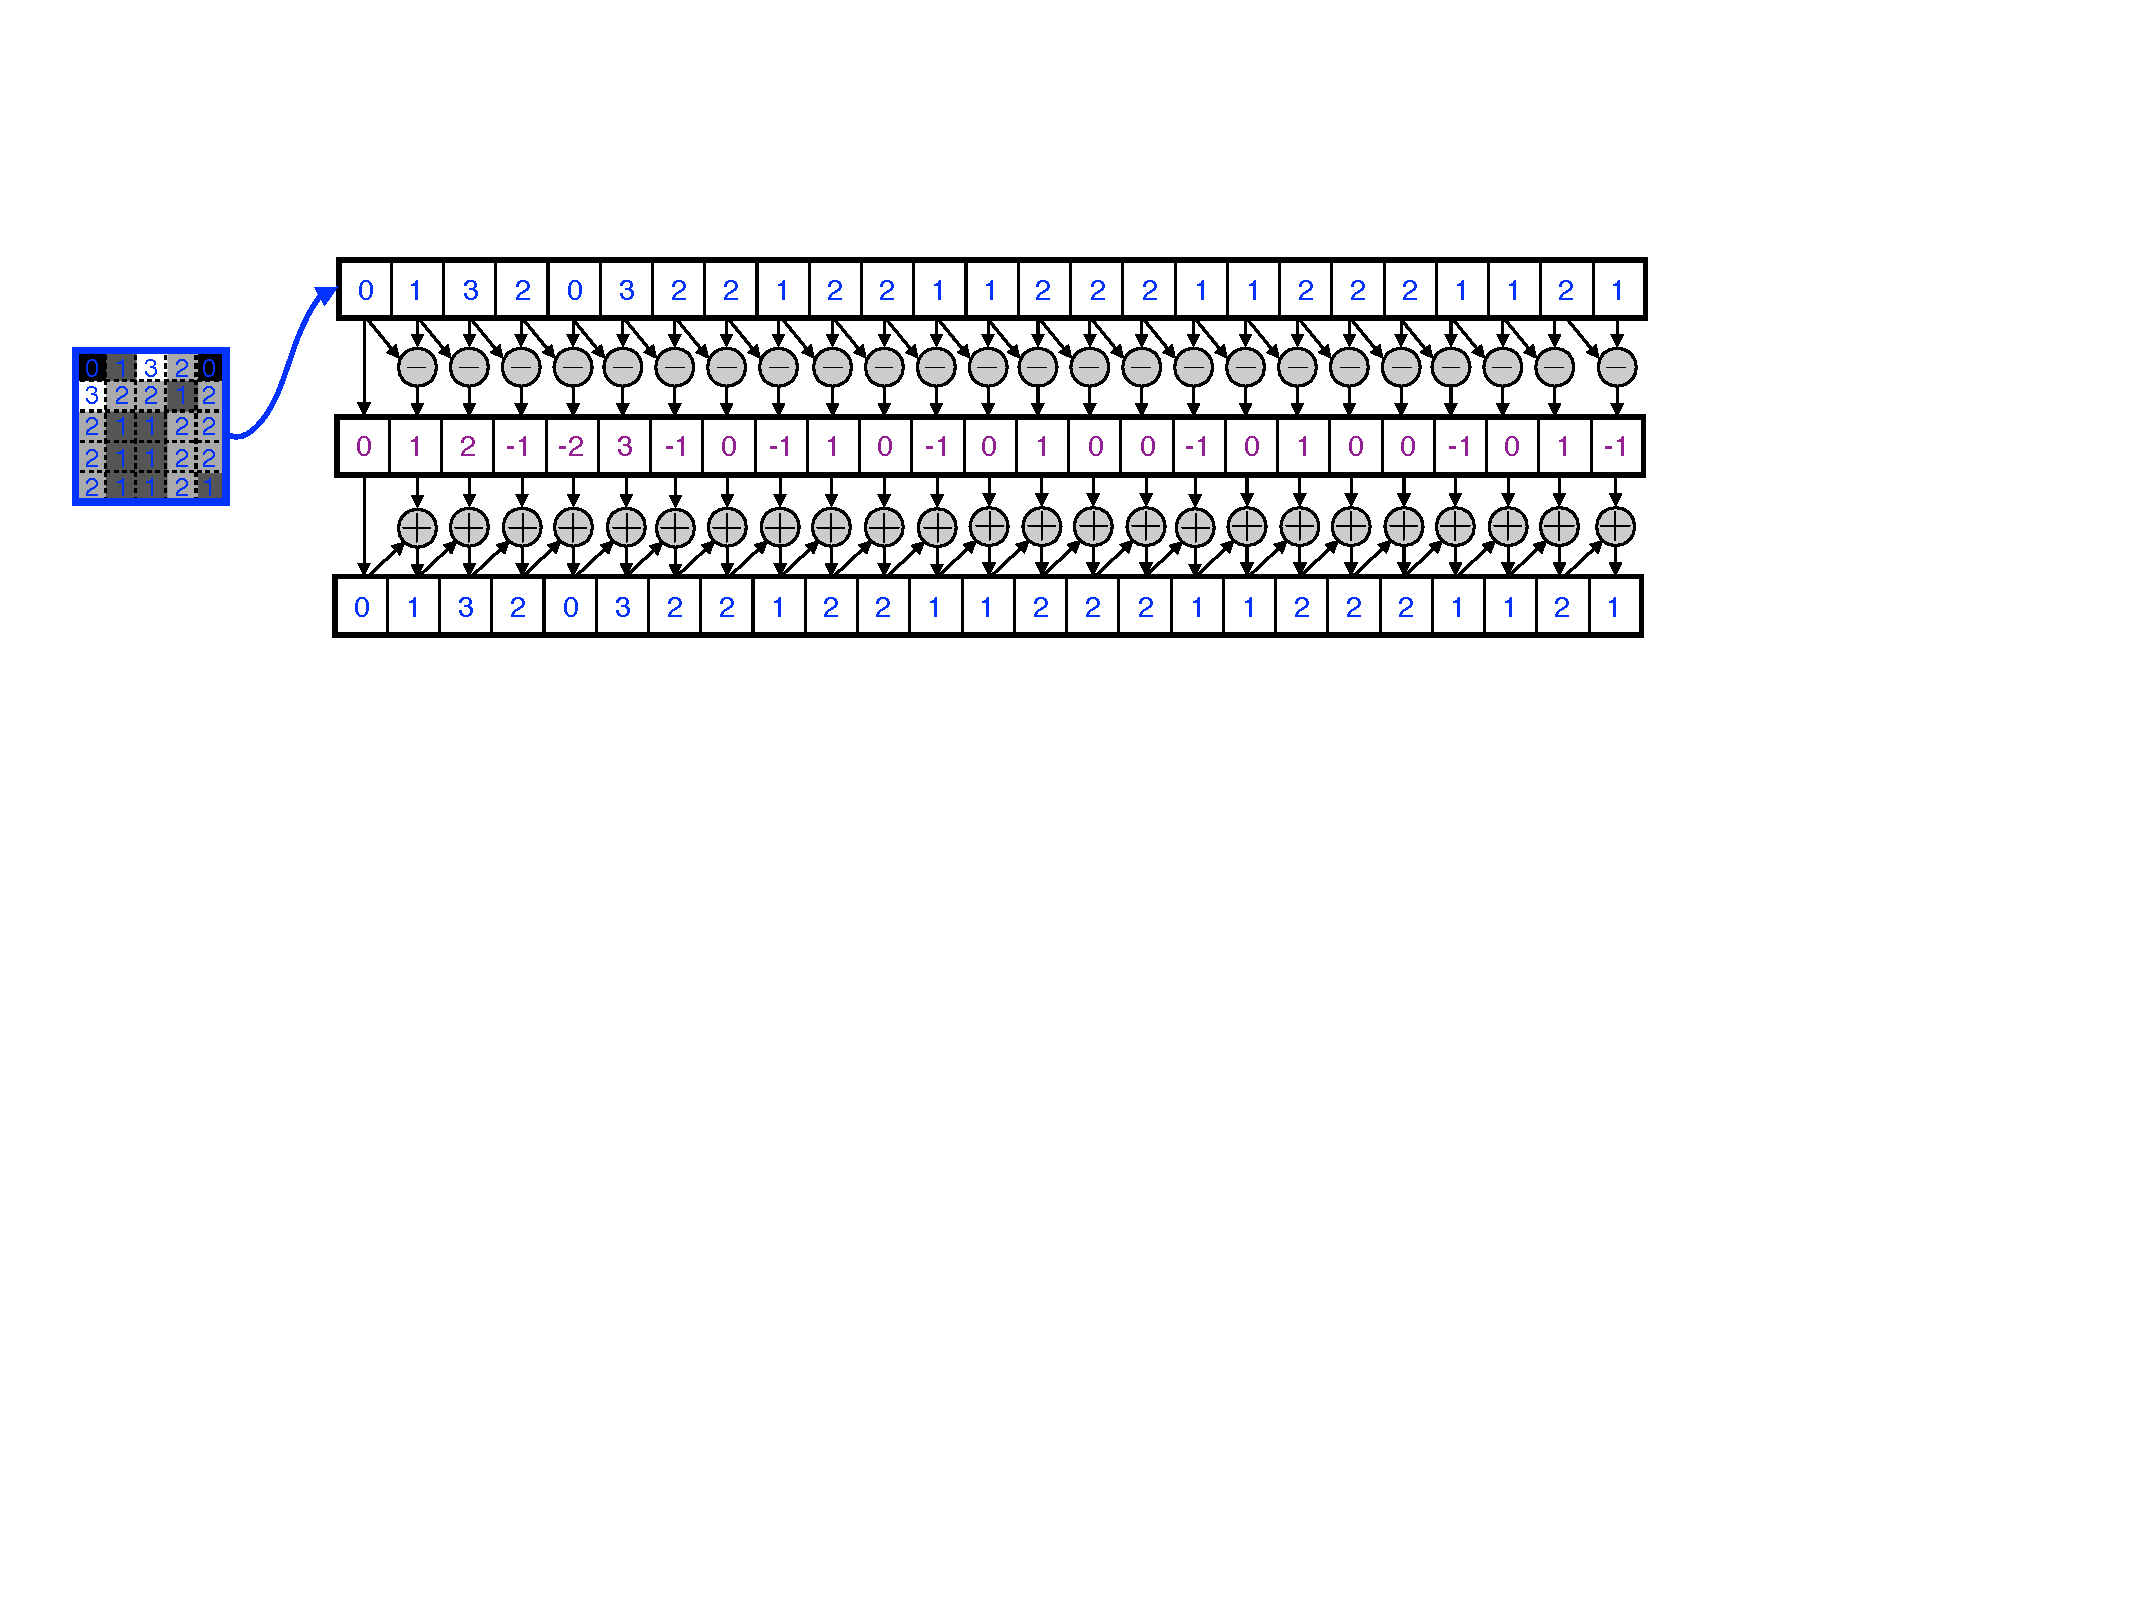
\includegraphics[width=\linewidth]{differences/differences}}
{fig-codage-differences}{Différences successives et reconstruction par sommation cumulée, en conservant le premier pixel.}

Pour l'image de la fleur, l'histogramme des différences est plus concentré que celui des pixels. Les entropies empiriques et les longueurs de Huffman de la figure~\ref{fig-entropy-differences} illustrent le gain obtenu en codant séparément les valeurs. Ce gain n'est pas garanti pour toute image.
\myfig{\tabTrois{
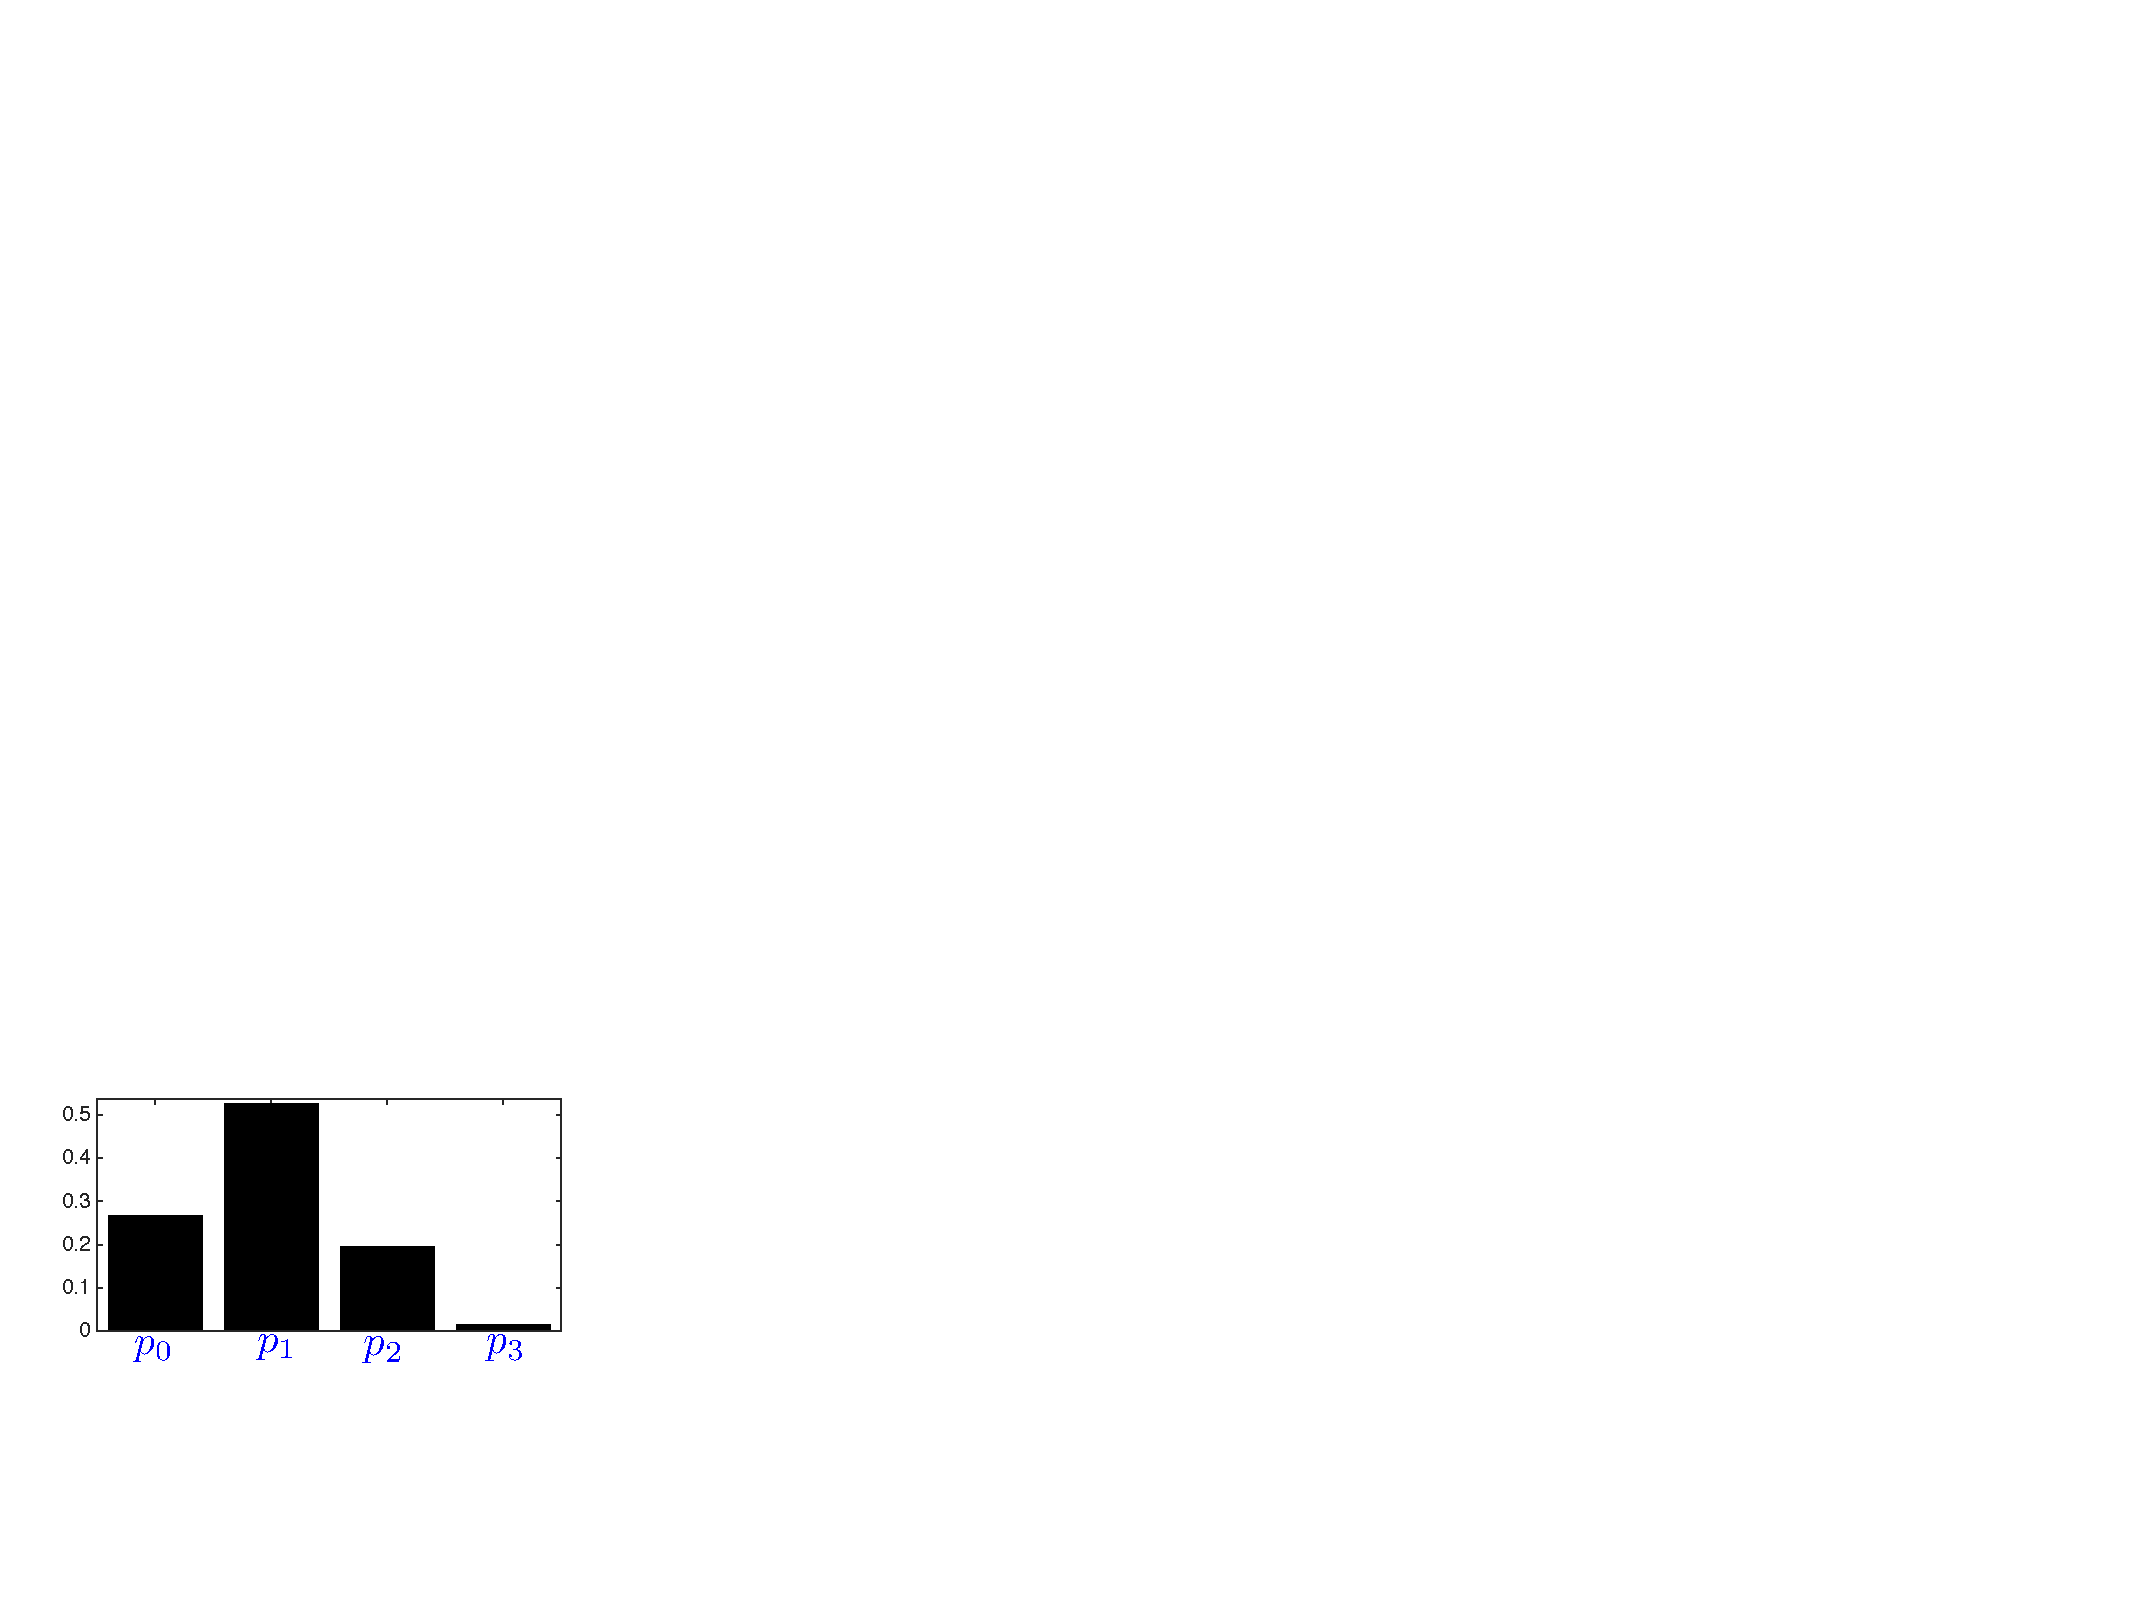
\includegraphics[width=.29\linewidth]{differences/histo-pix}&
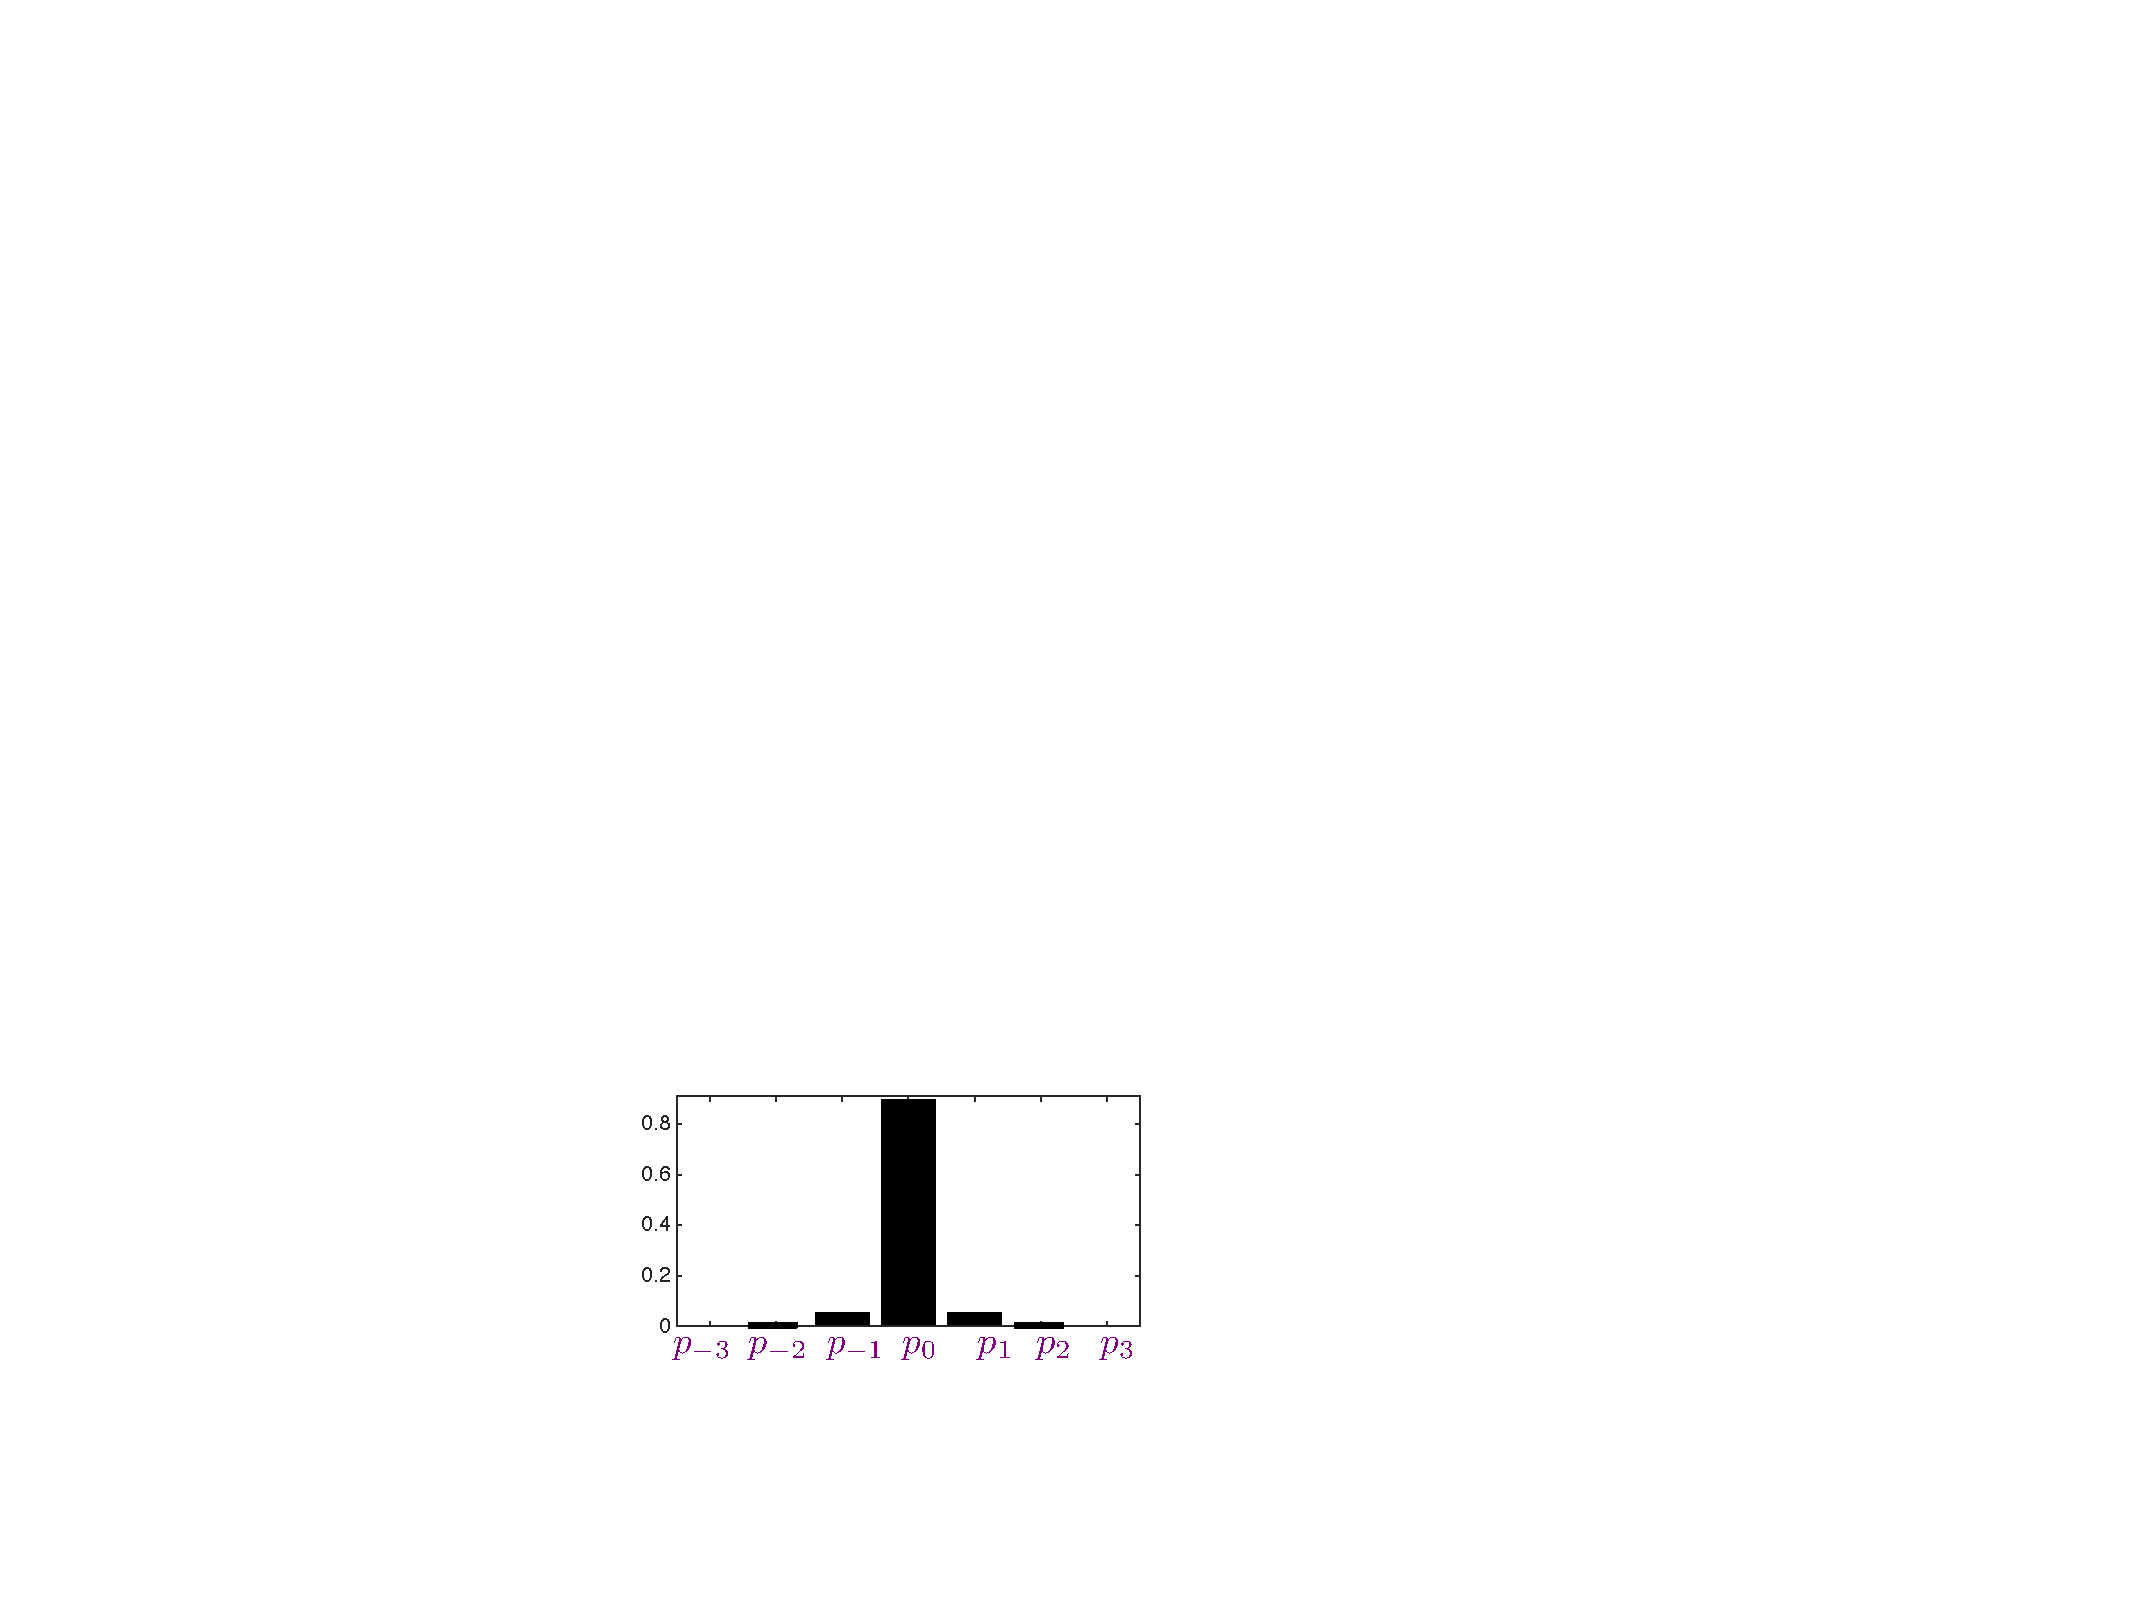
\includegraphics[width=.29\linewidth]{differences/histo-diff}&
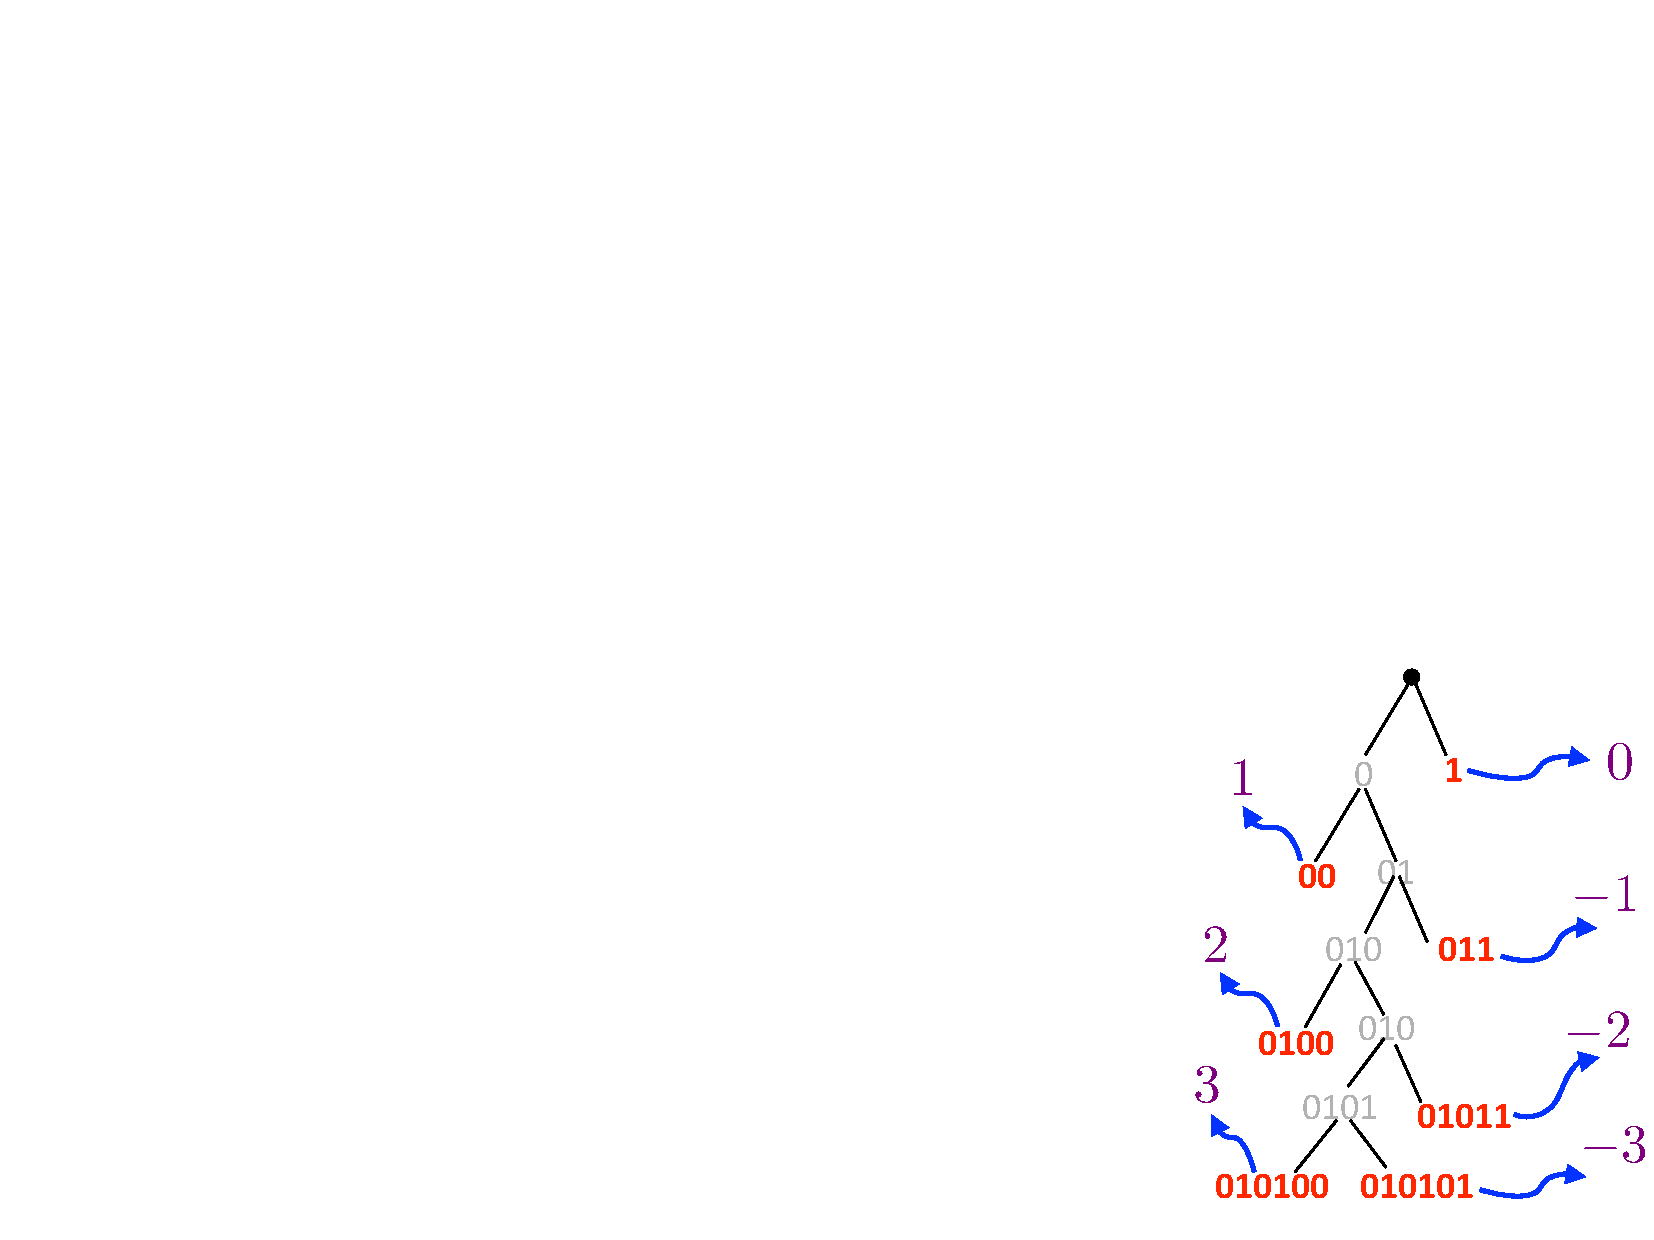
\includegraphics[width=.21\linewidth]{differences/arbre-difference}\\
$H\simeq1{,}54,\ L\simeq1{,}67$&$H\simeq0{,}61,\ L\simeq1{,}16$&\text{Arbre préfixe}}}
{fig-entropy-differences}{Histogrammes des pixels et des différences sur l'image entière, avec un arbre de codage préfixe des différences.}

Le code représenté est
\[
\begin{array}{c|rrrrrrr}
 d&-3&-2&-1&0&1&2&3\\\hline
 c_d&010101&01011&011&1&00&0100&010100
\end{array}
\]
et sa longueur moyenne est d'environ $1{,}16$ bit par différence. En utilisant les débits arrondis affichés pour une image de $256\times256$ pixels, on estime le contenu codé à $16$ Kio pour le code uniforme sur deux bits, $13{,}36$ Kio pour le codage direct des pixels et $9{,}28$ Kio pour le codage des différences. Un Kio vaut $1024$ octets, soit $8192$ bits. Il faut ajouter à la dernière estimation le premier pixel et la description de la table de codage.

Une transformation bijective ne réduit \emph{pas} l'entropie jointe du message entier. Elle peut rendre les modèles symbole par symbole plus efficaces en modifiant les distributions marginales et les dépendances. La borne~\eqref{eq-shannon-bound} ne requiert aucune hypothèse d'indépendance pour un symbole aléatoire pris isolément ; cette hypothèse a servi plus haut à obtenir $H(V_1,\ldots,V_n)=nH(V)$. Pour une source dépendante, c'est l'entropie jointe du bloc qui fournit la borne pertinente.

Les méthodes de compression d'images plus élaborées combinent prédiction ou transformations, quantification et codage entropique. JPEG 2000, par exemple, utilise les ondelettes et possède des modes avec et sans perte~\cite{mallat2009a-wav}. L'exploitation des dépendances s'applique également aux lettres d'un texte.

\paragraph*{Pour aller plus loin.}
On pourra consulter~\cite{CoverThomas} pour approfondir le codage de source et~\cite{mallat2009a-wav} pour ses applications au signal et à l'image. Les programmes des figures originales sont disponibles sur \url{https://github.com/gpeyre/2016-shannon-theory} ; d'autres expériences figurent dans les Numerical Tours~\cite{2011-peyre-cise}.

\ifdefined\StandaloneChapter
\par\noindent\begin{minipage}{\linewidth}
\section*{Glossaire}
\begin{multicols}{2}\small\raggedright
\begin{rs}
\gloss{Pixel} : emplacement dans la grille d'une image, ou valeur qui y est stockée.
\gloss{Symbole} : élément de l'alphabet fini à coder.
\gloss{Mot de code} : suite de bits associée à un symbole.
\gloss{Code} : correspondance entre les symboles et leurs mots de code.
\gloss{Distribution empirique} : fréquences relatives observées des symboles.
\gloss{Histogramme} : représentation graphique de ces fréquences.
\gloss{Modèle de source} : loi de probabilité des symboles ou de leurs suites.
\gloss{Entropie} : information moyenne $H(V)$, positive ou nulle, mesurée en bits.
\gloss{Longueur moyenne du code} : $L(c)=\sum_vp_v\ell_v$, en bits par symbole.
\end{rs}
\end{multicols}
\end{minipage}\par
\fi

\ifdefined\StandaloneChapter
\paragraph*{Remerciements.}
Je remercie Marie-Noëlle Peyré, Gwenn Guichaoua, François Béguin, Gérard Grancher, Aurélien Djament et François Sauvageot pour leurs relectures attentives. La photographie de la fleur est due à Maïtine Bergounioux.
\fi
